\begin{frame}{第二十四讲、定积分}
	\linespread{1.5}
	\begin{enumerate}
	  \item {\bf 内容与要求}{\b( \S 6.1 )}
	  \begin{itemize}
	    \item 理解定积分的概念与几何意义
% 	    \item 理解可积的基本条件
	    \item 熟练掌握定积分的基本性质
	    \item 理解定积分中值定理
	  \vspace{1em}
	  \end{itemize}
	  \item {\bf 课后练习:}
	  \begin{itemize}
	    \item 书面作业:{\b 习题6.1:3(1,3),4,5(4,5,6),6}
 	    \item 思考题:{\b 习题6.1:7,8,9,10}
	  \end{itemize}
	\end{enumerate}
\end{frame}

\section{定积分的基本概念}

\begin{frame}{问题的提出}
	\linespread{1.2}\pause 
	{\bf 问题:}如何求给定曲线所围平面区域的面积?\pause 
% 	\begin{itemize}
% 	  \item 土地丈量
% 	  \item 
% 	  \item 布料剪裁
% 	\end{itemize}
	\begin{columns}
		\column{.48\textwidth}
		\begin{block}{\bf 求“曲边梯形”的面积}
			给定曲线$y=f(x)$,求由该曲线及$y=0$,
			$x=a$,\\
			$x=b$所围区域的面积
		\end{block}
		\uncover<5->{$$\alert{S=\dint_a^bf(x)\d x}$$}
		\column{.52\textwidth}
		\begin{center}
			\uncover<4->{\resizebox{!}{5.2cm}{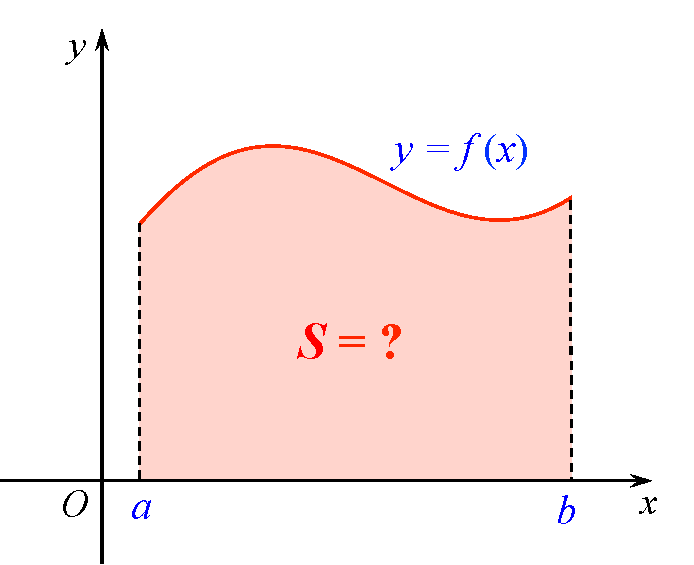
\includegraphics{./images/ch6/integral.pdf}}}
		\end{center}
	\end{columns}
\end{frame}

\begin{frame}{解决思路}
	\linespread{1.2}\pause 
	\begin{exampleblock}{{\bf 例1}\hfill P301}
		求由曲线$y=x^2$以及直线$x=0,x=1$和$y=0$所围成的曲边梯形的面积。
	\end{exampleblock}\pause 
	\begin{itemize}
	  \item {\bb 分割:}沿$x$轴方向分割曲边梯形\pause 
	  \item {\bb 取近似:}用小矩形的面积$S_i$近似小曲边梯形面积\pause 
	  \item {\bb 做和:}求所有小矩形的面积总和$\sum S_i$\pause 
	  \item {\bb 求极限:}$\sum S_i\to S$
	\end{itemize}
\end{frame}

\begin{frame}{定积分的定义}
	\linespread{1.2}\pause 
	\begin{block}{{\bf 定义6.1.1}\hfill P307}
		{\bb 函数$y=f(x)$在区间$[a,b]$上(Riemann)可积:}\pause 
		$$\dint_a^bf(x)\d x=\lim\limits_{\lambda\to
		0}\sum\limits_{k=1}^nf(\xi_k)\Delta x_k$$
	\end{block}\pause 
	\begin{itemize}
	  \item \alert{上式右端极限对$[a,b]$的任意分法均存在且相同}\pause 
	  \item \alert{$\lambda\to 0$用于保证分割得足够“细”}\pause 
	  \item \alert{给定分法,$\xi_k$的取法应该是任意的}
	\end{itemize}
\end{frame}

\begin{frame}
	\linespread{1.2}\pause 
	\begin{block}{{\bf 定理6.1.1}\hfill P308}
		\begin{enumerate}
		  \item $f(x)$在$[a,b]$上可积,则一定在$[a,b]$上有界\pause 
		  \item $f(x)$在$[a,b]$上连续,则一定在$[a,b]$上可积\pause 
		\end{enumerate}
	\end{block}
	\begin{itemize}
	  \item \alert{分段连续(只有有限个第一类间断点)的函数是可积的}
	\end{itemize}\pause 
	\begin{exampleblock}{{\bf 例2}\hfill P309}
		证明Dirichlet函数在任意区间$[a,b]$上不可积。
	\end{exampleblock}
\end{frame}

\section{定积分的几何意义}

\begin{frame}{定积分的几何意义}\pause 
	\linespread{1.2}
	\begin{itemize}
	  \item {\bb “带有符号的面积”}\pause 
	\end{itemize}
	\begin{center}
		\resizebox{!}{3.12cm}{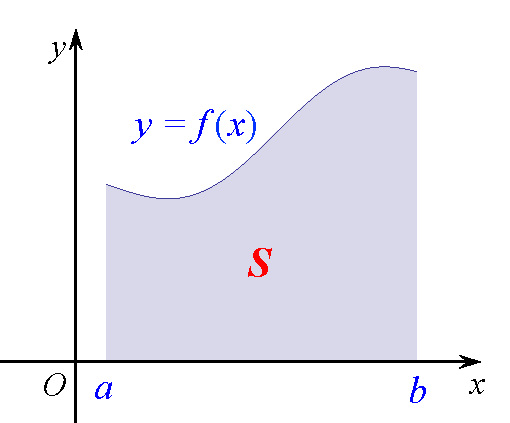
\includegraphics{./images/ch6/IS1.pdf}}\pause 
		\resizebox{!}{3.12cm}{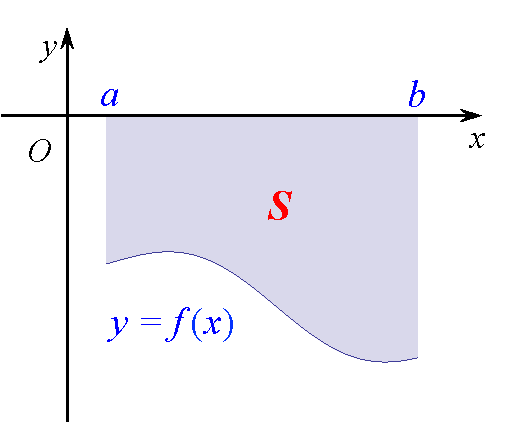
\includegraphics{./images/ch6/IS2.pdf}}\pause 
		\resizebox{!}{3.12cm}{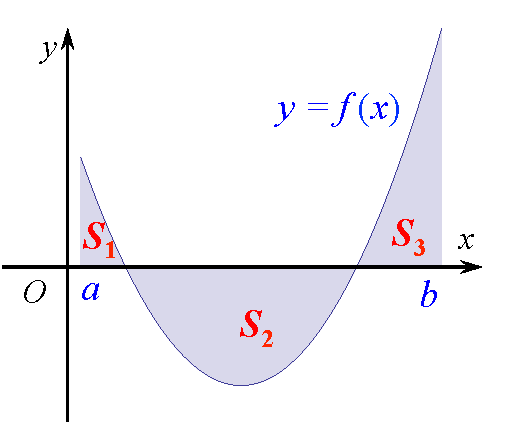
\includegraphics{./images/ch6/IS3.pdf}}\pause 
	\end{center}
	{\bf 约定:}\pause 
% 	\begin{block}{{\bf 约定}\hfill}
		\begin{columns}
			\column{.4\textwidth}
			\begin{enumerate}
			  \item \alert{$\dint_a^af(x)\d x=0$}\pause 
% 			  \item $\dint_b^af(x)\d x=-\dint_a^bf(x)\d x$
			\end{enumerate}
			\column{.6\textwidth}
			\begin{enumerate}
			  \addtocounter{enumi}{1}
% 			  \item $\dint_a^af(x)\d x=0$
			  \item \alert{$\dint_b^af(x)\d x=-\dint_a^bf(x)\d x$}
			\end{enumerate}
		\end{columns}
		
% 	\end{block}
\end{frame}

\section{定积分的基本性质}

\begin{frame}{定积分的基本性质}
	\linespread{1.2}\pause 
	\begin{block}{{\bf 定理}\hfill P310-316}
		\begin{enumerate}\pause 
		  \item {\bb 线性性:}
		  $$\dint_a^b[\alpha
		  f(x)+\beta g(x)]\d x=\alpha\dint_a^bf(x)\d x+\beta\dint_a^bg(x)\d x$$\pause 
		  \item {\bb 区间可加性:}
		  $$\dint_a^bf(x)\d x=\dint_a^cf(x)\d x+\dint_c^bf(x)\d x$$
		\end{enumerate}
	\end{block}
\end{frame}

\begin{frame}
	\linespread{1.2}
	\begin{block}{{\bf 定理}(续)\hfill P310-316}
		\begin{enumerate}\pause 
		  \addtocounter{enumi}{2}
		  \item {\bb 保号性:}\pause 
		  \begin{itemize}
		    \item $f(x)$在$[a,b]$上可积,且$f(x)\geq 0$,则$\dint_a^bf(x)\d x\geq 0$\pause 
		    \item $f(x)$在$[a,b]$上连续,非负且不恒为零,则$$\dint_a^bf(x)\d x> 0$$\pause 
		    \item {\bb 保序性:}设$f(x),g(x)$在$[a,b]$上可积,且$f(x)\leq g(x)$,则
		    $$\dint_a^bf(x)\d x\leq \dint_a^bg(x)\d x$$
		  \end{itemize}
		\end{enumerate}
	\end{block}
\end{frame}

\begin{frame}
	\linespread{1.2}
	\begin{block}{{\bf 定理}(续)\hfill P310-316}
		\begin{enumerate}
		  \addtocounter{enumi}{2}
		  \item {\bb 保号性:}(续)\pause 
		  \begin{itemize}
		    \item {\bb
		    绝对值不等式:}$f(x)$在$[a,b]$上可积,则$$\dint_a^bf(x)\d x\leq\dint_a^b|f(x)|\d x$$\pause 
		    \item {\bb 积分估值:}$f(x)$在$[a,b]$上可积,且$m\leq f(x)\leq M$,则
		    $$m(b-a)\leq\dint_a^bf(x)\d x\leq M(b-a)$$
		  \end{itemize}
		\end{enumerate}
	\end{block}
\end{frame}

\section{定积分中值定理}

\begin{frame}{定积分中值定理}\pause 
	\linespread{1.2}
	\begin{block}{{\bf 定理6.1.2}\hfill P314}
		若函数$f(x)$在区间$[a,b]$上连续,则在$[a,b]$上至少存在一点$\xi$,使得
		$$\dint_a^bf(x)\d x=f(\xi)(b-a)$$
	\end{block}\pause 
	{\ba{思考:}} 定积分中值定理与微分中值定理有何联系?
\end{frame}

\begin{frame}[<+->]{小结}
	\linespread{1.5}
	\begin{columns}
		\column{.5\textwidth}
		\begin{enumerate}
		  \item {\bf 定积分的概念}
		  \item {\bf 定积分的基本性质}
		  \begin{itemize}
		    \item 线性型
		    \item 区间可加性
		    \item 保号性
		    \item 保序性
		    \item 积分估值
		    \item 中值定理
		  \end{itemize}
		\end{enumerate}
		\column{.5\textwidth}
		\begin{center}
			\alert{定积分的几何意义}\\
			\resizebox{!}{5.2cm}{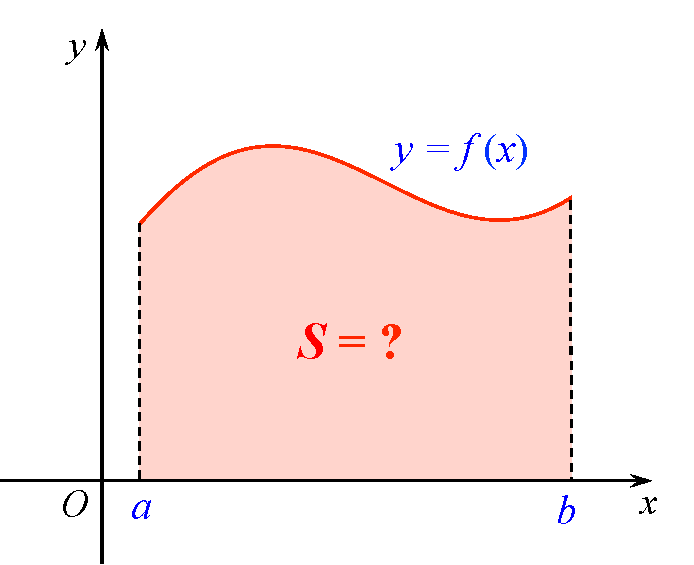
\includegraphics{./images/ch6/integral.pdf}}
		\end{center}
	\end{columns}
	
% 	\bigskip
% 	\pause
% 	\centerline{\ba{请自行阅读第六章\S 6.3节}}
\end{frame}

\begin{frame}{课堂练习}
	\linespread{2}
	\begin{exampleblock}{{\bf 例3}\hfill P317-习题7}
		将下列求和式表示成定积分\pause 
		\begin{enumerate}
		  \item $\limn\df 1n\left[\sin\df{\pi}{n}+\sin\df{2\pi}{n}+\ldots
		  +\sin\df{(n-1)\pi}{n}\right]$\pause 
		  \item $\limn\left(\df{1}{n^2}+\df{2}{n^2}+\ldots+\df{n-1}{n^2}\right)$
		\end{enumerate}
	\end{exampleblock}
\end{frame}

%======================================

% \begin{frame}{title}
% 	\linespread{1.2}
% 	\begin{block}{{\bf title}\hfill}
% 		123
% 	\end{block}
% \end{frame}